% !Rnw root = learnR.Rnw



\marginnote{For an overview of what is available under the R
  umbrella, see the CRAN Task View:
  \url{http://cran.csiro.au/web/views/Spatial.html}.}
In the past several years, there have been spectacular advances in R's
mapping and spatial analysis abilities. These have used R as a unfied
framework both for abilities that were developed within R and for
abilities that were designed to run independently of R.  Use of R in
this way can have huge benefits.

From the R command line, the relevant R packages can be installed thus:
\sidenote{Alternatively, install from the GUI menu.}
\begin{Schunk}
\begin{Sinput}
install.packages(c("rgdal","gstat","sp"),
                 dependencies=TRUE)
\end{Sinput}
\end{Schunk}

The {\em rgdal} binaries for Windows and for MacOS X include GDAL,
PROJ.4 and Expat. This avoids any need to install this software
outside of R. Ensure also that you have \txtt{rJava}.

\section{Static Overlay onto Maps}

\begin{Schunk}
\begin{Sinput}
library(oz)
library(DAAG)
\end{Sinput}
\end{Schunk}

\subsection{Overlay onto country and regional outlines}

Figure \ref{fig:possumsites} uses the function \txtt{oz()} in the
\textit{oz} package to plot an outline of the Australian coast and
state boundaries.

\begin{marginfigure}
\begin{Schunk}


\centerline{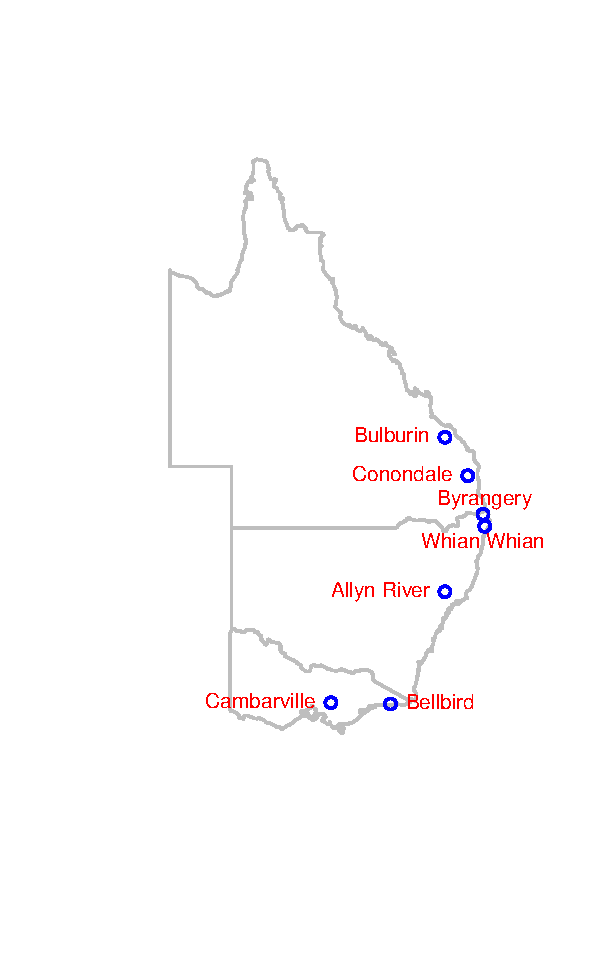
\includegraphics[width=0.47\textwidth]{figs/13-oz-sites-1} }

\end{Schunk}
\vspace*{-21pt}

\caption{Sites at which possums were collected.\label{fig:possumsites}}
\end{marginfigure}

Labeling information has been added, using the functions
\txtt{points()} and \txtt{text()}, that identifies seven sites where
studies of possums were conducted.  Names of sites, and latitude and
longitude information, were taken from the \txtt{possumsites} data
set.

Code used for plot is:
\begin{Schunk}
\begin{Sinput}
oz(sections=c(3:5, 11:16), col="gray")
chh <- par()$cxy[2]
with(possumsites, {
  points(Longitude,
         Latitude+c(0,0,0,.2,-.2, 0,0)*chh,
         col="blue")
  text(Latitude ~ Longitude,
       labels=rownames(possumsites),
       col="red", pos=c(2,4,2,1,3,2,2), xpd=TRUE)
  # pos = 1:below, 2:left, 3:above, 4:right
  # xpd=TRUE allows plotting outside figure region
})
\end{Sinput}
\end{Schunk}
% $

\subsection{The {\em dismo} package's Interface to Google maps}

The function \txtt{gmap()} ({\em dismo} package) is designed to 
access and download Google map data.

\marginnote{Loading the package {\em dismo}, with the default
  \txtt{dependencies=TRUE}, will at the same time load the {\em sp}
  and {\em raster} packages.}
\begin{Schunk}
\begin{Sinput}
library(dismo, quietly=TRUE)
  ## The raster and sp packages are dependencies
\end{Sinput}
\end{Schunk}

\paragraph{Basic syntax, accepting defaults:}
The following is a simple example of what is possible:
\marginnote{The argument \margtt{type} to \margtt{gmap()} can be 
set to \margtt{'roadmap'}, \margtt{'satellite'}, \margtt{'hybrid'}or
\margtt{'terrain'}.  Use \margtt{scale=2} to double the number of
pixels (default is 1.}

\begin{Schunk}
\begin{Sinput}
cbr <- gmap("Canberra, ACT")
plot(cbr)
acton <- gmap("Acton, ACT", type="satellite")
plot(acton)
\end{Sinput}
\end{Schunk}
Road addresses can be specified. Try, e.g.
\marginnote{The argument \margtt{zoom} takes values between 0 and 21.}
\begin{Schunk}
\begin{Sinput}
TBhouse <- gmap('11 Bowen St, Wellington, NZ',
                type='satellite', scale=2, zoom=20)
plot(TBhouse)
\end{Sinput}
\end{Schunk}

\paragraph{Specify map longitude/latitude extent; overlay onto map:}
The data frame \txtt{possumsites} ({\em DAAG}) holds latitudes and
longitudes of possum study sites.  In the
following, a map is created that takes in all the sites.  Site
names are then overlaid on to the map: \marginnote{Extents are
  specified in a longitude/latitude coordinate system.  The
  function \txtt{gmap()} will, unless called with \txtt{lonlat=TRUE},
  return a raster object that uses a Mercator projection.}
\begin{Schunk}
\begin{Sinput}
## Extend longitude & latitude ranges slightly
lonlat <- with(possumsites,
               c(range(Longitude)+c(-3,3),
                 range(Latitude)+c(-2,2))
)
## Obtain map, as a ``RasterLayer'' object
googmap <- gmap(extent(lonlat))
plot(googmap, inter=TRUE)
## From latitude/longitude to Mercator projection
xy <- Mercator(with(possumsites,
                    cbind(Longitude, Latitude)))
## Points show location of sites on the map
points(xy)
## Add labels that give the names
text(xy, labels=row.names(possumsites))
\end{Sinput}
\end{Schunk}

\paragraph{Interactive selection of a map extent from a screen display:}
Type:
\begin{Schunk}
\begin{Sinput}
newlims <- drawExtent()
\end{Sinput}
\end{Schunk}
Now click at opposite corners\sidenote{An initial click on the map may
be required to initiate the process.}  of the rectangular region
that is to be selected.  Red '+' symbols will appear at the locations
clicked, and a bounding box will be marked out in red.  Then enter:
\marginnote{The new area is likely to be somwhat larger than was
marked out by the bounding box.}
\begin{Schunk}
\begin{Sinput}
googmap2 <- gmap(newlims)
plot(googmap2)
\end{Sinput}
\end{Schunk}

\subsection{The {\em plotKML} package}

\begin{Schunk}
\begin{Sinput}
require(plotKML)
\end{Sinput}
\end{Schunk}

The \txtt{plotKML()} function overlays any of points, lines, contours
and images onto a Google earth display.  Just as with a standard
Google Earth display, this can be manipulated with a mouse or
trackpad.  The following brings the data into R:
\marginnote{The range of dates is from 2009-08-02 to 2014-01-20,
  for quakes of magnitude 4.5 or greater.
  Subsection |ref{ss:markup} has the code that was used
  to retrieve the data from the NZ GeoNet website.}
\begin{Schunk}
\begin{Sinput}
library(DAAGviz)
fullpath <- system.file('datasets/nzquakes.CSV',
                        package='DAAGviz')
quakes <- read.csv(fullpath)
quakes$Date <- as.Date(quakes$Date)
quakes$Energy <- 10^quakes$magnitude/1000000
\end{Sinput}
\end{Schunk}

Now prepare the data for plotting:
\begin{Schunk}
\begin{Sinput}
## Prepare data for plotting
coordinates(quakes) <- ~ longitude+latitude
proj4string(quakes) <-
  CRS("+proj=longlat +datum=WGS84")
\end{Sinput}
\end{Schunk}

Now create the display:
\marginnote{If the image does not appear, look in the working directory
for {\bf quakes\_\_Energy\_\_.kml}, and click on it.}
\begin{Schunk}
\begin{Sinput}
plotKML(quakes['Energy'], points_names="")
  # Makes circle area proportional to Energy
\end{Sinput}
\end{Schunk}

\subsection{Specifying projections}
Note that we had to specify a coordinate system.  With
longitude/latitude coordinates, as above, we can specify
\txtt{"WGS84"}. Projections become important when spatial data, e.g.,
on metal concentrations, is overlaid on map data, e.g., from Google
maps.  See \txtt{help(proj4string)} and \txtt{help(CRS)} for further
details.

\section{Working with Raster (Image) Files}
\marginnote{Among the many raster formats
are several that are widely used for image files more
generally: BMP, various JPEG formats, GIF, PNG, XPM, etc.
Georeferencing, allowing inclusion of spatial reference data,
is available for BMP, JPEG 2000 formats, and TIFF.}
The function \txtt{readGDAL()} in the {\em rgdal} package is
intended for reading GDAL grid maps.
The following, loosely based on the example code in the help pages for
\txtt{readGDAL}, requires the packages {\em rgdal}, {\em sp}, and
       {\em grid}.  We begin by using the function \txtt{readGDAL()}
to input, as a grid, the R logo file that is supplied with the
R package \txtt{rgdal}:
\begin{Schunk}
\begin{Sinput}
library(rgdal)
logofile <- system.file("pictures/Rlogo.jpg",
                        package = "rgdal")[1]
rlogo <- readGDAL(logofile, silent=TRUE)
\end{Sinput}
\end{Schunk}
Typing these commands from the command line, but with
\txtt{silent=FALSE}, will result in the warning message ``GeoTransform
values not available''.  This is not surprising.  The pixels in the
image do not have associated geographical spatial coordinates.

Now examine the input object:
\begin{Schunk}
\begin{Sinput}
class(rlogo)
\end{Sinput}
\begin{Soutput}
[1] "SpatialGridDataFrame"
attr(,"package")
[1] "sp"
\end{Soutput}
\begin{Sinput}
names(rlogo)
\end{Sinput}
\begin{Soutput}
[1] "band1" "band2" "band3"
\end{Soutput}
\end{Schunk}
\noindent
Observe that the file has been input as a \txtt{SpatialGridDataFrame}. The
function \txtt{image} has a method for objects of this class.

The command \txtt{image()}, specifying the red, green and blue channels,
can be used to show the figure, using the folowing code:

\begin{Schunk}
\begin{Sinput}
image(rlogo, red="band1",
      green="band2",
      blue="band3")
\end{Sinput}
\end{Schunk}
\noindent
The function \txtt{spplot.grid()} is called to do the plotting.
In turn, it calls function \txtt{levelplot()} from the
{\em lattice} package.

Another possibility is to use the function \texttt{spplot()}
  to examine the red green and blue layers separately, as in Figure
  \ref{fig:rlogo3}:
\begin{figure}
\begin{Schunk}


\centerline{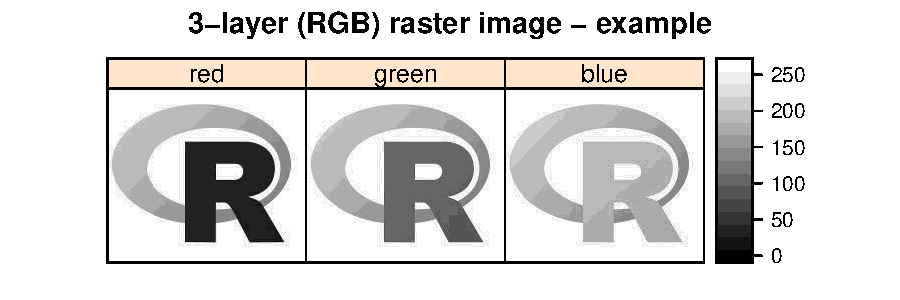
\includegraphics[width=0.47\textwidth]{figs/13-spplot-col3-1} }

\end{Schunk}
\caption{Red, green and blue layers from the R logo image.\label{fig:rlogo3}}
\end{figure}
\begin{Schunk}
\begin{Sinput}
## Code
col3 <- c("red","green","blue")
spplot(rlogo, zcol=1:3, names.attr=col3,
       col.regions=grey(0:100/100), as.table=TRUE,
       layout=c(3,1), main=paste("3-layer (RGB)",
       "raster image - example"))
\end{Sinput}
\end{Schunk}

  Note also the functions \txtt{spplot.polygons()} and
  \txtt{spplot.points()}.  These are all documented on the same page
  as the generic function \txtt{spplot()}.

\subsection*{$^*$A genuine spatial image}

The following locates the file that will be input
from the package installation directory:
\begin{Schunk}
\begin{Sinput}
sp27 <- system.file("pictures/SP27GTIF.TIF",
                    package = "rgdal")[1]
\end{Sinput}
\end{Schunk}

Now use \txtt{readGDAL()} to create a GDAL grid map image:
\begin{marginfigure}
The following can be used to get information about the file,
before inputting it:
\begin{Schunk}
\begin{Sinput}
GDALinfo(sp27)
\end{Sinput}
\end{Schunk}
\end{marginfigure}
\begin{Schunk}
\begin{Sinput}
SP27GTIF <- readGDAL(sp27, output.dim=c(100,100),
                     silent=TRUE)
class(SP27GTIF)
\end{Sinput}
\begin{Soutput}
[1] "SpatialGridDataFrame"
attr(,"package")
[1] "sp"
\end{Soutput}
\end{Schunk}
Then to plot the image, enter:
\begin{Schunk}
\begin{Sinput}
spplot(SP27GTIF)
\end{Sinput}
\end{Schunk}

\subsection{Overlaying onto a bubble plot}

\begin{marginfigure}
\begin{Schunk}


\centerline{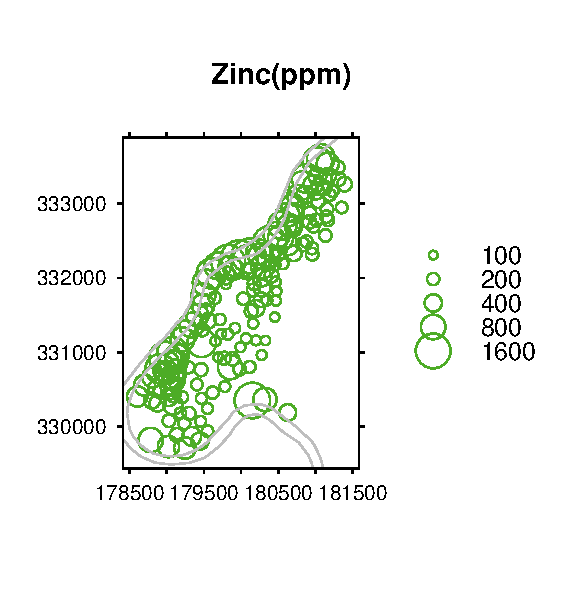
\includegraphics[width=0.98\textwidth]{figs/13-meuse-bubble-1} }

\end{Schunk}
\vspace*{-15pt}
 \caption{Bubble plot for \margtt{zinc},
with area of bubbles proportional to concentration.
River Meuse boundaries are in gray.\label{fig:ZnRiv}}
\end{marginfigure}

Figure \ref{fig:Znbubble} in Section \ref{ss:S4} showed how to use a
bubble plot to display the \txtt{meuse} data from the \txtt{sp}
package.  Figure \ref{fig:ZnRiv} adds river boundaries, using data from the
dataset \txtt{meuse.riv}.  (This is a matrix, with Eastings in column
1 and Northings in column 2.)

The function \txtt{bubble()} uses the abilities of the {\em lattice}
package. As a consequence, the layering abilities of the {\em
  latticeExtra} package (see Subsection \ref{ss:panel}) can be used to
add to the plot. Code is:


\begin{Schunk}
\begin{Sinput}
library(sp)
data(meuse); data(meuse.riv)
coordinates(meuse) <- ~ x + y
gph <- bubble(meuse, "zinc", pch=1, key.entries =  100 * 2^(0:4),
              main = "Zinc(ppm)", scales=list(axes=TRUE, tck=0.4))
add <- latticeExtra::layer(panel.lines(meuse.riv[,1], meuse.riv[,2],
                      col="gray"))
gph+add
\end{Sinput}
\end{Schunk}

{\small
\section{$^*$Reading and Processing Shapefiles}
Shapefiles (ESRI Shapefiles) are a popular geospatial vector data
format.  For detailed comments, see
\url{http://en.wikipedia.org/wiki/Shapefile}.  They describe
geometries -- points, lines and polygons.

The subdirectory {\bf vectors}, stored as part of the {\em rgdal}
package, has a number of shapefile collections.  The following
extracts and stores the path (dsn = ``dataset name'') to this
directory:
\begin{Schunk}
\begin{Sinput}
dsn <- system.file("vectors", package = "rgdal")[1]
dir(dsn, pattern="shp$")
\end{Sinput}
\begin{Soutput}
[1] "cities.shp"                   "kiritimati_primary_roads.shp"
[3] "scot_BNG.shp"                 "trin_inca_pl03.shp"          
\end{Soutput}
\end{Schunk}
\noindent
There are thus three shapefile collections, or ``layers''.
\begin{marginfigure}
  The following can be used to get information on the \txtt{"cities"}
layer, prior to input:
\begin{Schunk}
\begin{Sinput}
ogrInfo(dsn=dsn,
        layer="cities")
\end{Sinput}
\end{Schunk}
\end{marginfigure}

The files in the \txtt{cities} shapefile collection are:
\begin{Schunk}
\begin{Sinput}
## Get names of files in shapefile collection
dir(dsn, pattern="cities")
\end{Sinput}
\begin{Soutput}
[1] "cities.dbf" "cities.htm" "cities.prj" "cities.sbn" "cities.sbx"
[6] "cities.shp" "cities.shx"
\end{Soutput}
\end{Schunk}
The mandatory files are the {\bf .shp} (shape format), the {\bf .shx}
(shape index format) and {\bf .dbf} (attribute format) files.  For
  detailed information, see
  \url{http://en.wikipedia.org/wiki/Shapefile}.
\marginnote{Note also {\bf .prj} files, which hold coordinate
  system and projection information.}

Now input the shapefile collection {\bf cities}:
\begin{Schunk}
\begin{Sinput}
cities <- readOGR(dsn=dsn, layer="cities", verbose=FALSE)
\end{Sinput}
\end{Schunk}
\noindent
The \txtt{readOGR()} function combines information from the separate
shapefiles into a \txtt{SpatialPointsDataFrame}

The following gives summary information:
\begin{Schunk}
\begin{Sinput}
summary(cities)
\end{Sinput}
\begin{Soutput}
Object of class SpatialPointsDataFrame
Coordinates:
              min   max
coords.x1 -165.27 177.1
coords.x2  -53.15  78.2
Is projected: FALSE 
proj4string :
[+proj=longlat +datum=WGS84 +no_defs +ellps=WGS84 +towgs84=0,0,0]
Number of points: 606
Data attributes:
        NAME        COUNTRY      POPULATION  CAPITAL
 Hyderabad:  2   US     : 49   -99    : 30   N:442  
 San Jose :  2   Russia : 37   1270000:  5   Y:164  
 Tripoli  :  2   China  : 36   1550000:  4          
 Valencia :  2   Canada : 22   1140000:  3          
 Abidjan  :  1   India  : 20   1190000:  3          
 Abu Zaby :  1   Brazil : 19   1225000:  3          
 (Other)  :596   (Other):423   (Other):558          
\end{Soutput}
\end{Schunk}
\noindent
The four ``data attributes'' are columns of the \txtt{data} slot.  Use
for example \txtt{cities\$COUNTRY} or \txtt{cities[,"COUNTRY"]} to
extract the column \txtt{COUNTRY}.  \marginnote{For example, omne
  might add, using data on the World Bank website, a column giving the
  percentage of the population under 20 years of age.}  Further
columns can be added as required, or existing columns removed or
modified.

To get information obout the countries represented, type:
\begin{Schunk}
\begin{Sinput}
slotNames(cities)
\end{Sinput}
\begin{Soutput}
[1] "data"        "coords.nrs"  "coords"      "bbox"        "proj4string"
\end{Soutput}
\begin{Sinput}
names(cities)
\end{Sinput}
\begin{Soutput}
[1] "NAME"       "COUNTRY"    "POPULATION" "CAPITAL"   
\end{Soutput}
\begin{Sinput}
  ## Returns the names in the data slot
length(levels(cities$COUNTRY))
\end{Sinput}
\begin{Soutput}
[1] 165
\end{Soutput}
\end{Schunk}
\noindent
There are 165 countries.

The following extracts and plots the shapefile details for Canada:
\begin{Schunk}
\begin{Sinput}
canada <- subset(cities, COUNTRY=="Canada")
trellis.par.set(sp.theme())
spplot(canada, zcol="POPULATION")
\end{Sinput}
\end{Schunk}

\subsection*{ASGC Digital Boundaries}

The following downloads, to the working directory, a zipfile for
a directory that holds 2011 statistical region boundaries in ESRI
shapefile format:
\begin{Schunk}
\begin{Sinput}
url <- paste0("http://www.abs.gov.au/ausstats/subscriber.nsf/",
  "log?openagent&1259030001_sr11aaust_shape.zip&1259.0.30.001",
  "&Data%20Cubes&B8003880BC09FA5BCA2578CC00124E25&0",
  "&July%202011&14.07.2011&Latest")
download.file(url, destfile="../downloads/1259030001_sr11aaust_shape.zip")
\end{Sinput}
\end{Schunk}
\noindent
The file is 25.6MB and, depending on the speed of the connection,
will take a modest time to download.

Alternatively, go to the web page
  \url{http://www.abs.gov.au/AUSSTATS/abs@.nsf/DetailsPage/1259.0.30.001July%202011?OpenDocument},
    locate the zip file identified as containing ``Statistical
    Region ASGC Ed 2011 Digital Boundaries in ESRI Shapefile Format'',
    and download it.  Click on SUMMARY to get information that
    describes the codes that are used to identify states and
    territories, the field headers, ans the nature of the included
    data.

% The code chunks that follow assume that the file has been
% successfully downloaded.
The following then unzips the files into the
subdirectory {\bf au-srs}:
\marginnote{If the file is not in the working directory, precede the
  file name with the path to the file.}
\begin{Schunk}
\begin{Sinput}
unzip("../downloads/1259030001_sr11aaust_shape.zip", exdir="au-srs")
dir("../downloads/au-srs")
\end{Sinput}
\begin{Soutput}
[1] "SR11aAust.cpg" "SR11aAust.dbf" "SR11aAust.prj" "SR11aAust.shp"
[5] "SR11aAust.shx"
\end{Soutput}
\end{Schunk}

Now input the information from the shapefiles, and combine
it to create a \txtt{SpatialPolygonsDataFrame}, named \txtt{auSRS},
that has statistical region boundaries:
\begin{Schunk}
\begin{Sinput}
auSRS <- readOGR("../downloads/au-srs", layer="SR11aAust")
\end{Sinput}
\begin{Soutput}
OGR data source with driver: ESRI Shapefile 
Source: "../downloads/au-srs", layer: "SR11aAust"
with 66 features
It has 3 fields
\end{Soutput}
\end{Schunk}
States or territories are 1:New South Wales, 2:Victoria, 3:Queensland,
4:South Australia, 5:Western Australia, 6:Tasmania, 7:Northern Territory,
8:Australian Capital Territory, 9:Other Territories.
The following extracts the \txtt{SpatialPolygonsDataFrame} for Victoria.
\begin{Schunk}
\begin{Sinput}
vicSRS <- subset(auSRS, STATE_CODE==2)
unique(vicSRS@data[,"SR_NAME11"])
\end{Sinput}
\begin{Soutput}
 [1] Outer Western Melbourne   North Western Melbourne  
 [3] Inner Melbourne           North Eastern Melbourne  
 [5] Inner Eastern Melbourne   Southern Melbourne       
 [7] Outer Eastern Melbourne   South Eastern Melbourne  
 [9] Mornington Peninsula      Barwon-Western District  
[11] Central Highlands-Wimmera Loddon-Mallee            
[13] Goulburn-Ovens-Murray     All Gippsland            
66 Levels: All Gippsland ... Wide Bay-Burnett
\end{Soutput}
\end{Schunk}
\noindent
Notice that all 66 factor levels from \txtt{auSRS} have been retained,
even though only 14 of these levels are present in this dataset.

Functions are available for combining files of this type, or for
removing boundaries such as between the \txtt{SR\_NAME11} regions.

\subsection*{Further information}
The R geo website, at \url{http://www.r-project.org/Rgeo/} has extensive
information.  The Wiki page
\url{http://spatial-analyst.net/wiki/index.php?title=Software} has
extensive information about installation of relevant geostatistical
software.

Table 3.1 in Hengl(2011) compares the
  spatio-temporal abilities of some popular statistics and GIS
  packages.  There are columns for R+{\em gstat} and R+{\em geoR.}

The web page
\url{http://www.nceas.ucsb.edu/scicomp/usecases/ReadWriteESRIShapeFiles}
has several examples that demonstrate the reading and plotting of
shapefiles, comparing abilities in the {\em rgdal} package with those
in {\em maptools} and {\em PBSmapping}. Note also the package
{\em shapefiles}.

The website
\url{http://info.geonet.org.nz/display/appdata/Earthquake+Web+Feature+Service}
has information on how New Zealand earthquake data may be retrieved in
a variety of formats.
The site \url{http://www.christchurchquakemap.co.nz/} has impressive
dynamic visualizations of Christchurch (NZ) and other quake data.

A carefully documented example of the use of shapefiles of New Zealand
data can be found at\newline
\noindent
\url{http://www.r-bloggers.com/simplifying-polygon-shapefiles-in-r/}.
}
\section{Other software -- QGIS}
Note in particular QGIS, which has an interface via {\em manageR} to
R; go to \url{http://www.ftools.ca/plugins.html}.

To obtain Windows and Linux installers for QGIS, go to
\url{http://www.qgis.org/wiki/Download}.  The standalone installer for
Windows includes GRASS.  For MacOSX, go to
\url{http://www.kyngchaos.com/software/qgis}.  For Leopard and Snow Leopard
installations, the QGIS 1.7 developer builds seem relatively stable.
GRASS must be installed separately.

\section{References}

\begin{itemize}
\item[] Bivand R, Pebesma E J, Gomez-Rubio, V. 2008. Applied Spatial Data
Analysis with R.  Springer.
\item[] Diggle, Peter J. \& Ribeiro Jr, Paulo J 2007. Model-Based Geostatistics.
Springer.
\item[] Hengl, T. 2011, A Practical Guide to Geostatistical
  Mapping. 2nd edn.\newline
[To download (free) or purchase (\$US15.19), go to:\\
\url{http://www.lulu.com/} and search for 'Hengl']
\item[] Hijmans, R J. 2011. Introduction to the 'raster' package.\newline
[With the R package {\em raster} attached, type \txtt{vignette("Raster")}.
\item[] Hijmans, R J and Elith J. 2011. Species distribution modeling with R.\newline
[With the R package {\em dismo} attached, type \txtt{vignette("sdm")}.
The vignette appears to be an outline for a book.  Later chapters are
very incomplete.]
\item[] Lamigueiro, O P 2012. Maps with R (I)
\url{http://procomun.wordpress.com/2012/02/18/maps_with_r_1/}
\item[] Maindonald, J H 2011.  Generalized Additive Models in Spatial
  Statistics -- Linear Models with a Twist (slides).
\url{maths.anu.edu.au//~johnm/r/spatial/}\newline
[This offers a perspective on spatial interpolation.]
\item[] Quantum GIS Development Team 2010.  Quantum GIS User Guide(
  Version 1.6.0 `Copiap\'{o}').  Obtain from
\url{http://www.qgis.org/en/documentation/manuals.html}
\end{itemize}
See also the vignettes that accompany the package {\em sp}, describing
classes and methods for spatial data, and overlay and aggregation.
